% REMEMBER: You must not plagiarise anything in your report. Be extremely careful.

\documentclass{l4proj}

    
%
% put any additional packages here
%

\begin{document}

%==============================================================================
%% METADATA
\title{Work in Progress Title: Investigations in Learning Analytics}
\author{Elisabet Tammjarv}
\date{September ??, 2024}

\maketitle

%==============================================================================
%% ABSTRACT
\begin{abstract}
    Every abstract follows a similar pattern. Motivate; set aims; describe work; explain results.
    \vskip 0.5em
    ``XYZ is bad. This project investigated ABC to determine if it was better. 
    ABC used XXX and YYY to implement ZZZ. This is particularly interesting as XXX and YYY have
    never been used together. It was found that  
    ABC was 20\% better than XYZ, though it caused rabies in half of subjects.''
\end{abstract}

%==============================================================================

% EDUCATION REUSE CONSENT FORM
% If you consent to your project being shown to future students for educational purposes
% then insert your name and the date below to  sign the education use form that appears in the front of the document. 
% You must explicitly give consent if you wish to do so.
% If you sign, your project may be included in the Hall of Fame if it scores particularly highly.
%
% Please note that you are under no obligation to sign 
% this declaration, but doing so would help future students.
%
\def\consentname {Elisabet Tammjarv} % your full name
\def\consentdate {23 December 2023} % the date you agree
%
\educationalconsent


%==============================================================================
\tableofcontents

%==============================================================================
%% Notes on formatting
%==============================================================================
% The first page, abstract and table of contents are numbered using Roman numerals and are not
% included in the page count. 
%
% From now on pages are numbered
% using Arabic numerals. Therefore, immediately after the first call to \chapter we need the call
% \pagenumbering{arabic} and this should be called once only in the document. 
%
% Do not alter the bibliography style.
%
% The first Chapter should then be on page 1. You are allowed 40 pages for a 40 credit project and 30 pages for a 
% 20 credit report. This includes everything numbered in Arabic numerals (excluding front matter) up
% to but excluding the appendices and bibliography.
%
% You must not alter text size (it is currently 10pt) or alter margins or spacing.
%
%
%==================================================================================================================================
%
% IMPORTANT
% The chapter headings here are **suggestions**. You don't have to follow this model if
% it doesn't fit your project. Every project should have an introduction and conclusion,
% however. 
%
%==================================================================================================================================
\chapter{Introduction}

% reset page numbering. Don't remove this!
\pagenumbering{arabic} 

\section{Description of Problem}

\subsection{Overview of Learning Analytics}
Learning analytics (LA) is broadly defined as the measurement, collection, analysis, and reporting of data about learners and learning environments - with the main purpose consisting of gaining an insight into the interactions between learners and the systems they participate in \citep{Papamitsiou2014InternationalEvidence}. LA encompasses a plethora of conceptual variations with its multi-disciplinary approach that ties together areas of education, psychology, computing and data science \citep{Ifenthaler2020UtilisingReview}. In line with our student-centred philosophy for LA (discussed in section !!!!), we will be focusing on applications of LA which operate on a strictly institutional level. 

*******ADD CATEGORIES OF LA USE CASES HERE.*********

\section{Motivation}


\section{Aim}


    

%==================================================================================================================================
\chapter{Background}
What did other people do, and how is it relevant to what you want to do?
\section{Research Concerns for Learning Analytics}
First, a short disclaimer. The majority of papers written on LA lack an underlying theoretical framework, resulting in an inherent lack of ability to connect findings with meaningful pedagogical guidance \citep{Baek2023Educational2019, Banihashem2019InvestigationAnalytics, BuchnerPersonalisedModel}. The field also suffers from a lack of rigorous, large-scale evidence for the effectiveness of LA implementations in learning environments \citep{Ifenthaler2020UtilisingReview}. The use of LA to provide evidence of detecting various constructs relevant to learners and education suffers from a lack of replicability, in part due to the large degree of freedom in research for decisions made regarding content analysis as well as the highly contextual nature of the data itself \citep{Kitto_Manly_Ferguson_Poquet_2023}. The often sensitive nature of datasets for LA leads to a restrictive model wherein companies and research groups with access to larger, closed datasets tend to excel - thereby narrowing the reproducibility of results within the field \citep{Kitto_Manly_Ferguson_Poquet_2023}. With these doubts in mind, I have carefully reviewed my research for this literature review and organised the key findings into four overarching categories;- deviance within underlying motivations for the implementation of LA projects, deviance within developmental methods undertaken, deviance within the implementation of the projects, and finally the interplay of ethics and law in LA. 


\section{Literature Review}
\subsection{Underlying Motivations}
The underlying motivations behind why projects with LA have been created affect everything from the resilience and usefulness of the system down to how it is interpreted by the users themselves. The use of LA to identify learners who are at risk of dropping out can directly increase profits for an institution, and opting for data-driven optimization rather than expert oversight is often viewed as a cost-cutting measure \citep{Yen-TingLiuLearningPoint}. This can alienate educators from their practices as well as their students. Predictive LA, in particular, has been viewed as a form of behaviourism, with learners' behaviour being influenced by institutes that claim to have their best interests at heart \citep{Yen-TingLiuLearningPoint}. The unfortunate reality of cases where LA has gone awry is that institutions are often too large, complicated and teeming with other projects to manage each high-risk case individually - and when there is no clear-cut trail of responsibility, the blame is put on the implementations, and use of,
LA itself. LA has been heading in a similar direction as AI and Big Data faddism, grasping the attention of institutes as an easy solution for dealing with otherwise abstract and difficult problems \citep{BeerThreeAustralia}. 


\subsection{Developmental Methods}
\subsubsection{Stakeholders}

Most LA projects are developed with an educator-centric institutional view, with learners relegated to acting as passive end-users \citep{Joseph-Richard2023WhichPerspective}. On the flip side, learner-centric, learner-led LA projects are often performative in nature, with strong emphasis placed on the outcome of learners' educational paths over the learning process itself; this simultaneously discourages lower self-efficiency learners and encourages complacency within high-achieving students \citep{Yen-TingLiuLearningPoint}. \citet{BeerThreeAustralia} explore how the development of Learning Analytics (LA) systems with a focus on educator-centric, institutional views can be influenced by the diverse ways educators are involved in the process. Three approaches are discussed:

1. Top-Down: This involves forming and considering a project at the institutional level with input from a small group before implementing it institution-wide.

2. In-Group: Here, a project is initiated and utilized by a passionate group of educators who may not be aware of the significant differences between the in-group and the majority of educators in the institute. 

3. Bricolage: In this approach, a project is developed by first understanding the existing resources and working with educators to gain insights into their lived experiences. 

The paper ends by mentioning a mixture of elements in all three approaches is the best, despite the top-down approach being the existing institutional norm.

Another important factor for us to consider is the clear divergences in stakeholders' perspectives over bias and equity reflected by the institutional position they hold, i.e. learners have comparatively limited awareness of details surrounding LA implementations but still express concerns over the use of their data - whilst few educators and administrators see students as active and trustworthy partners in managing their data \citep{Heiser2023AmplifyingEducation}. \citet{Heiser2023AmplifyingEducation} further discusses how the fragmentation that can occur amongst stakeholders can be mitigated, with a focus on centring the values of different stakeholder groups whilst acknowledging intersections and power dynamics between groups for authentic inclusion. 

\subsubsection{Course Structure}
Differences present in course structure can make or break the usefulness of LA projects \citep{Azevedo2017LearningLearning, Barberà_Gregori_Galvan_Fernandez_Zhang_Fernández-Navarro_2017, Iglesias-Pradas2015AssessingCompetencies}. To put this into perspective, a course that focuses more on in-person learning elements, such as seminars and group projects, will result in far less available data to analyze than a course that has weekly online submissions for coursework as well as quizzes. At-risk learners may not be picked up on until it is far too late. Educators with a preference for tools outside of the standard for their institute, as well as constantly changing API for third-party software that allows data collection, both pose issues for the resilience of LA projects. Maintenance can be quite the pickle. Providing up-to-date documentation of the project with malleability and capacity for complexity in data coded in is key for the evolution and adaption of LA projects, as tools used by educators, as well as underlying educational theory, are continuously advanced. As \citet{Zemsky_2014} describes, the curriculum in institutional higher education is often disconnected from its true goal of preparing post-secondary learners for the future, due to a miscellany of courses taught by educators passionate about their specific subject for which learners often settle for what is convenient. True education is substantially more than the sum of its parts - and LA projects often fail to capture that nuance. 

\subsubsection{Learner Expectations}
There are numerous support features that learners expect from LA; most of which can be sorted into the three general phases of self-regulation \citep{Panadero_2017, Dwiarie2023PersonalizedAnalytics}

\section*{Forethought Phase:}

\begin{enumerate}
    \item \textbf{Understanding the Capital T Task:}
        \begin{itemize}
            \item General learning path visualization.
            \item End goal visualization.
            \item Task instruction visualization.
            \item Output criteria visualization.
        \end{itemize}
        
    \item \textbf{Motivation Exploration:}
        \begin{itemize}
            \item Personalized recommendation features based on learning interest, learners initial level of capabilities, outcome expectancies, and goal orientation for the future career journey.
        \end{itemize}
\end{enumerate}

\section*{Performance Phase:}

\begin{enumerate}
    \item \textbf{Time Management and Task Challenges:}
        \begin{itemize}
            \item Information for time prioritization.
            \item Prompts to break down goals.
            \item Reminders for the target.
        \end{itemize}
        
    \item \textbf{Tracking Learning Activities and Progress:}
        \begin{itemize}
            \item Recording and tracking features for:
                \begin{itemize}
                    \item Learning activities (e.g., time spent, active rate, completion status).
                    \item Progress of learning goals.
                    \item Observation of peers' learning activities progress.
                \end{itemize}
        \end{itemize}
        
    \item \textbf{Efficient Access to Information:}
        \begin{itemize}
            \item Traces to highlight information.
            \item Recommendations based on:
                \begin{itemize}
                    \item Interest keywords.
                    \item Popularity.
                \end{itemize}
        \end{itemize}
        
    \item \textbf{Help-Seeking for Social Support:}
        \begin{itemize}
            \item Recommendations to connect with resourceful experts or peers.
            \item Functions to support psychological safety (e.g., anonymous options).
        \end{itemize}
        
    \item \textbf{Regulating Emotions and Motivation:}
        \begin{itemize}
            \item Gamification elements (e.g., leaderboard, reward points).
            \item Personalized notifications for motivational messages.
        \end{itemize}
        
    \item \textbf{Constructing New Knowledge:}
        \begin{itemize}
            \item Prompt and direct feedback to rehearse information.
            \item Features to stimulate self-learning.
            \item Reminder notifications to review and revisit materials.
        \end{itemize}
\end{enumerate}

\section*{Self-Reflection Phase:}

\begin{enumerate}
    \item \textbf{Self-Evaluation Challenges:}
        \begin{itemize}
            \item Self-evaluation analytics features based on various standards, including:
                \begin{itemize}
                    \item Certain targeted output criteria.
                    \item Group performance without competition aspects.
                    \item Own standards or past performance track record.
                    \item Review from experts.
                    \item Review from peers or other references.
                    \item Recommendations on future improvement and learning goals.
                \end{itemize}
        \end{itemize}
        
    \item \textbf{Concerns about Data Ethics:}
        \begin{itemize}
            \item Need for information on Data Privacy, Data Transparency, and Data Security.
            \item Awareness of what data is acquired, for what purpose, and how it is secured.
        \end{itemize}
        
    \item \textbf{Data Privacy and Security:}
        \begin{itemize}
            \item Students expressing concerns about sharing personal data.
            \item Request for information on data acquisition, purpose, and security.
        \end{itemize}
        \BlankLine
\end{enumerate}


Prior assessments of learners' preferences indicate learners are interested in LA projects containing; a timeline showing current status and goals, reminders for deadlines, real-time written feedback for course materials as well as on the progression of learners' educational pathways, analysis and comparison of learners' learning style compared to peers, recommendation system for learning partners, time expected to complete tasks and read texts, support for timekeeping, planning and organising studies, adaptive recommendation of resources with a linked rating scale, personalized analysis of learners task and time management, recording and tracking of their learning activities, functionality to support psychological safety such as anonymity, analytic features to stimulate excitement for learners, prompts to help learners engage in the overall construction of new knowledge, additional help in assessing learner's needs for objective self-evaluation \citep{Schumacher2018FeaturesAnalytics}. There is also growing interest in challenging institutional reliance on measurable digital footprints as proxies for academic success by taking into account qualitative narratives, self-directed learning data, social networking models and personal financial data for resource utilization \citep{Joseph-Richard2023WhichPerspective}. As \citet{Joseph-Richard2023WhichPerspective} states; "Displaying data on the money making potential of courses or how much money is spent on fees in comparison with, for example, the extent to which they used the library sources, motivates 40\% of our participants. This information when presented with the data about other students’ economic behaviors appears to be a powerful motivator of success.".

\subsection{Implementation}
\subsubsection{Trust}
Perhaps the most crucial factor to consider for a successful implementation of an LA project is its trustworthiness. Third-party LA projects suffer from low levels of trust due to concerns around the privacy of data, use of outdated materials, and lack of governance in the aforementioned data \citep{ShannanAlzahrani2023DoStudy}. In-house LA projects suffer from low levels of trust due to missing transparency regarding the data use, viable project usefulness, and lack of belief in the competence of the institute \citep{ShannanAlzahrani2023DoStudy}. Analytics literacy is a key component in the belief of the project's usefulness, as users can easily misunderstand the use cases of the project and the limitations involved \citep{Feldstein_2017}. \citet{Papamitsiou2014InternationalEvidence} conducted SWOT analysis of LA projects shows human judgement as a major weakness of implemented LA projects, suggesting that the average user may have to acquire a specific skill set to be able to interpret results shown correctly. The complexity of intricate LA projects can result in a lack of generality for the results and an increased potential for the misclassification of patterns \citep{Papamitsiou2014InternationalEvidence}. These challenges contribute to conflicting findings regarding trust in the implementation of LA systems \citep{Papamitsiou2014InternationalEvidence}.

\subsubsection{Relationship Changes}
There are pedagogical concerns surrounding the transformation of student-educator, student-tutor, and student-course content relations due to LA and the use of technology for education in general \citep{Yen-TingLiuLearningPoint, Tempelaar2017AcceptedAssessment, Agudo-Peregrina2014CanLearning}. These concerns arise from their intrusion into individuals' private lives, as the boundaries between learning spaces and homes \citep{Baek2023Educational2019}. Another cause for concern is when the holistic nature of learning is not taken into account; perceived risk within a course is viewed as an independent variable, with dependent variables factors such as lecture attendance, active learning, motivation, prior academic performance and social connection \citep{Ifenthaler2020UtilisingReview}. This lack of contextualization within the bigger picture is exactly why during the COVID-19 pandemic measures of interaction were recorded and flagged as factors for poor performance across multiple institutes, for students to ‘fix’, without addressing the damaging effects that isolation in lockdown had on members of the student population. As a direct result of this breach of common sense, many educators critique LA by focusing on the importance of human presence \citep{MerikkoTechnologicalProcess}.

\subsubsection{Self Regulation}
Human presence is shown to be a significant factor for learners' success; with self-efficiency in social networking positively correlating to active academic help-seeking as well as an increased social presence within the learning environment \citep{Keshavarzi2023MediatingEnvironments}. Similarly, learners self-belief in their academic abilities positively correlates with their use of online services to help comprehend, organize and finalize their assessments \citep{Keshavarzi2023MediatingEnvironments}. The bridge between both of these skills, self-regulation, can be supported by LA projects taking the guise of pedagogical agents; scaffolding the responsibility and the skill set required for self-regulation from the LA project onto the learner themselves \citep{MerikkoTechnologicalProcess}. This must be done with careful consideration, demonstrated by the use of structured learning diaries by \citet{MerikkoTechnologicalProcess} for their LA project; whilst the diaries proved to successfully capture cognitive, emotional and motivational aspects of the self-regulation journey of learners, it harmed the self-regulation habits of a sub-group of students. When planning LA projects with the capacity to intervene in the self-regulation of learners, all three phases of self-regulation must be carefully taken into account; preparation, performance and appraisal \citep{Heikkinen123SupportingReview}. 

\subsubsection{Behaviourism}
Historically self-regulation, alongside other socio-emotional skills, was thought of as separate from personality traits; personality traits were fixed and socio-emotional skills could be changed with intervention. This is now considered inaccurate. Personality psychology can be used to accurately predict learners' educational outcomes, inform the basis of educational interventions and overall support academic development in learners \citep{Jach123HowResearch}. Learners personality traits can be used as target outcomes for students on their educational path, i.e. for a student struggling with coursework due to their first-year new place anxiety, working on lowering neuroticism (potential for anxiety and depression) and increasing agreeableness (potential for pro-social attitudes and behaviours) could be beneficial \citep{Jach123HowResearch}. If utilized within a LA project, personality trait tracking should be done with an extreme degree of caution, transparency to learners, and expert advice from the psychology field, since it is behaviourism; without the right accompanying elements, its usage does not focus on learners cognitive skills, carries limited application towards complex learning, does not care for individualization and increases potential for negative emotional impact by reinforcing the presence of traits that the learner sees as undesirable \citep{Tprestianni_2023}.


 
\subsection{Ethics and Law}

\subsubsection{Data Gathering}
Ethical conundrums surrounding the handling of big data focus on de-contextualization; and how it links to questionable claims of objectivity and generality - to combat this data handling must be transparent, personalized, networked, transportable, adaptive and interactive \citep{BeattieCreepyRights}. The potential LA has to further along the digital divide (the gap between demographics and regions with access to technological advancements and those without) must also be addressed \citep{BeattieCreepyRights}. What data we handle is also important; as there is strong evidence to suggest that the common practice of analyzing access log patterns has limited educational value, with potential benefits present for learners from deeper analyses of complex data \citep{Dietrichson2013BeyondPedagogies}. Combining qualitative data taken from various forms of assignments along with qualitative analysis can provide a more nuanced perspective \citep{Martinez2023Content-FocusedData}. This also has the benefit of potentially empowering learners' initiative for their education journey. Despite the hesitancy among learners to discuss sensitive information about themselves and their learning process, there is a demand for LA-based support for those topics \citep{MerikkoTechnologicalProcess}. Often learners, and educators, can hold mistaken assumptions about the value of individual learning processes - perhaps this is where the aforementioned hesitancy comes from. 


\subsubsection{Borderline Creep Factor}
We've all had the mutual moment of understanding as analytics moves from the territory of something useful and uncannily accurate to something that is deemed 'creepy analytics' by many; a colloquial that describes the invasion of data analytics upon the private lives of individuals. This can involve a lack of explicit consent and transparency regarding the process; much like when you click 'accept all' on Google and realize that you are now in the digital filter bubble matrix of marketing, forever \citep{Arthur_2013}. Creepy analytics within the field of LA stems from pervasive data collection methods such as biometrics and geopositioning, inherent human bias reflected within algorithms, intrusive predictions, and network mapping, all of which are uncomfortable and have the potential to violate learners boundaries \citep{BeattieCreepyRights}. The collection of big data on learners leaves them vulnerable to harm from hackers as well as malfeasance and misfeasance within the institute \citep{Daniel2016BigPractice}. The practice of utilizing LA for data-driven grading criteria has particularly unethical consequences that impact sub-groups of learners \citep{DimopoulosCONFERENCEPerformance}. As \citet{Sclater2016DevelopingAnalytics} demonstrates, creating a code of practice for assigning responsibility within institutions is key to avoiding introducing the 'creep factor' into LA projects.

\subsubsection{Responsibility}
The assignment of responsibility introduces its slew of paradoxical demands for those lucky enough to find themselves in charge; individuals may become burdened by an intense desire to clearly define the ethics behind their area, collecting as much data and analyzing the issue as far as is possible \citep{Lee2023ItsProgram}. The need to understand all aspects of concerns and problem-solve is a human instinct, but not everything falls into the realm of reason. In \citet{Lee2023ItsProgram} most mentors chose not to disclose information learned through LA about their mentees to their mentees. Although the mentors had taken the burden of responsibility for the mentee's educational pathways, they were unwilling to discuss why, and actions taken by mentors based on LA could not be aptly explained to mentees - causing conflict and changing the mentor's perceptions of their role. Mentor attention also focused on practices directly improving their mentee's scores, leaving mentees missing out on the rich variety of practices mentors and mentees would otherwise engage with. 

***********************LAW PART TO ADD TO*****************************

\section{Summary}

My review of pre-existing literature has highlighted the requirement for an underlying theoretical framework, and in line with my aims of supporting student self-regulation, I will be utilizing \citet{zimmerman2009self} theory of self-regulation as the foundational framework. Due to the constraints of this project, I will not be able to provide any rigorous, large-scale evidence for the effectiveness of LA implementations; however, I hope to provide a prototype showcasing the learner's interface for an institute-wide LA project, working alongside learners whilst utilizing agile methodologies. Careful consideration of data handling due to the fluid nature of ethics and law regarding LA, the differences present in structure across courses, and the evolution of educational theory needs to also be taken into account, with built-in flexibility and support for the growth of the LA project.  Learners may require additional material to improve their analytics literacy. The project should also have a strong focus on establishing and growing connections among learners, educators and course content. Analysis of potential benefits and consequences around utilizing personality trait analyses should be conducted before deciding if it will continue to be included in the design. Learners have substantial, varied expectations from LA support features, but are wary of creepy practices and breaches of privacy. Learners need to have full control over their data, as well as full transparency over the process. What one learner is willing to compromise on, another is not, and this will also have to be taken into account. Assessing responsibility is critical for LA projects, however the assignment of responsibility may lead to conflicts and changing perceptions of roles for learners and educators.

%==================================================================================================================================
\chapter{Analysis/Requirements}
What is the problem that you want to solve, and how did you arrive at it?
\section{Guidance}
Make it clear how you derived the constrained form of your problem via a clear and logical process. 

%==================================================================================================================================
\chapter{Design}
How is this problem to be approached, without reference to specific implementation details? 
\section{Guidance}
Design should cover the abstract design in such a way that someone else might be able to do what you did, but with a different language or library or tool.

%==================================================================================================================================
\chapter{Implementation}
What did you do to implement this idea, and what technical achievements did you make?
\section{Guidance}
You can't talk about everything. Cover the high level first, then cover important, relevant or impressive details.



\section{General points}

These points apply to the whole dissertation, not just this chapter.



\subsection{Figures}
\emph{Always} refer to figures included, like Figure \ref{fig:relu}, in the body of the text. Include full, explanatory captions and make sure the figures look good on the page.
You may include multiple figures in one float, as in Figure \ref{fig:synthetic}, using \texttt{subcaption}, which is enabled in the template.



% Figures are important. Use them well.
\begin{figure}
    \centering
    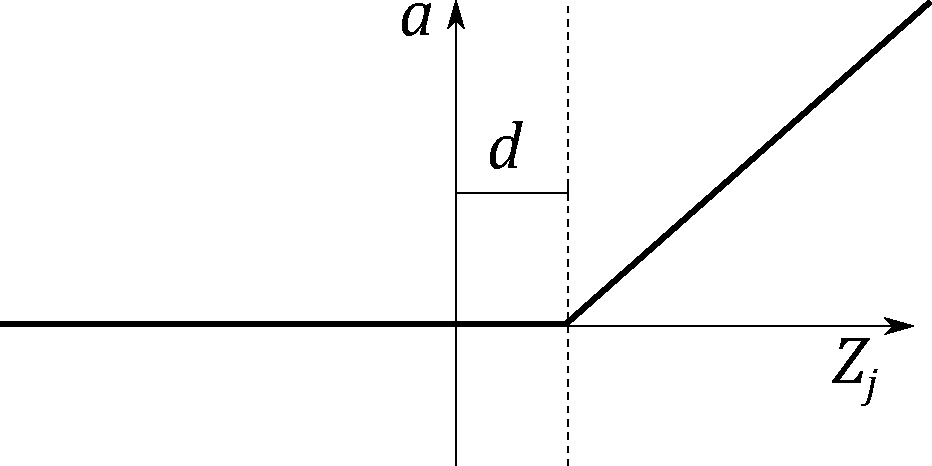
\includegraphics[width=0.5\linewidth]{images/relu.pdf}    

    \caption{In figure captions, explain what the reader is looking at: ``A schematic of the rectifying linear unit, where $a$ is the output amplitude,
    $d$ is a configurable dead-zone, and $Z_j$ is the input signal'', as well as why the reader is looking at this: 
    ``It is notable that there is no activation \emph{at all} below 0, which explains our initial results.'' 
    \textbf{Use vector image formats (.pdf) where possible}. Size figures appropriately, and do not make them over-large or too small to read.
    }

    % use the notation fig:name to cross reference a figure
    \label{fig:relu} 
\end{figure}


\begin{figure}
    \centering
    \begin{subfigure}[b]{0.45\textwidth}
        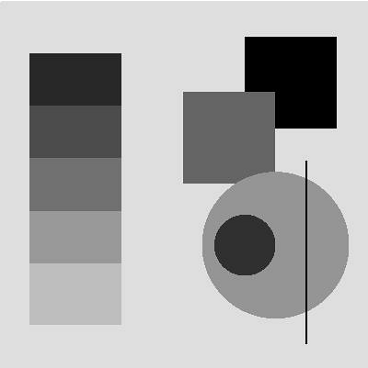
\includegraphics[width=\textwidth]{images/synthetic.png}
        \caption{Synthetic image, black on white.}
        \label{fig:syn1}
    \end{subfigure}
    ~ %add desired spacing between images, e. g. ~, \quad, \qquad, \hfill etc. 
      %(or a blank line to force the subfigure onto a new line)
    \begin{subfigure}[b]{0.45\textwidth}
        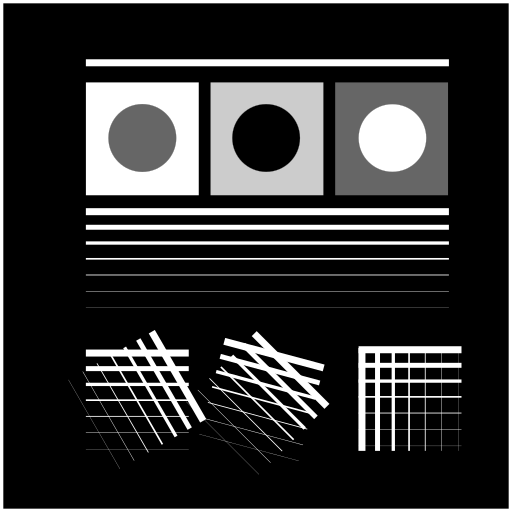
\includegraphics[width=\textwidth]{images/synthetic_2.png}
        \caption{Synthetic image, white on black.}
        \label{fig:syn2}
    \end{subfigure}
    ~ %add desired spacing between images, e. g. ~, \quad, \qquad, \hfill etc. 
    %(or a blank line to force the subfigure onto a new line)    
    \caption{Synthetic test images for edge detection algorithms. \subref{fig:syn1} shows various gray levels that require an adaptive algorithm. \subref{fig:syn2}
    shows more challenging edge detection tests that have crossing lines. Fusing these into full segments typically requires algorithms like the Hough transform.
    This is an example of using subfigures, with \texttt{subref}s in the caption.
    }\label{fig:synthetic}
\end{figure}

\clearpage

\subsection{Equations}

Equations should be typeset correctly and precisely. Make sure you get parenthesis sizing correct, and punctuate equations correctly 
(the comma is important and goes \textit{inside} the equation block). Explain any symbols used clearly if not defined earlier. 

For example, we might define:
\begin{equation}
    \hat{f}(\xi) = \frac{1}{2}\left[ \int_{-\infty}^{\infty} f(x) e^{2\pi i x \xi} \right],
\end{equation}    
where $\hat{f}(\xi)$ is the Fourier transform of the time domain signal $f(x)$.

\subsection{Algorithms}
Algorithms can be set using \texttt{algorithm2e}, as in Algorithm \ref{alg:metropolis}.

% NOTE: line ends are denoted by \; in algorithm2e
\begin{algorithm}
    \DontPrintSemicolon
    \KwData{$f_X(x)$, a probability density function returing the density at $x$.\; $\sigma$ a standard deviation specifying the spread of the proposal distribution.\;
    $x_0$, an initial starting condition.}
    \KwResult{$s=[x_1, x_2, \dots, x_n]$, $n$ samples approximately drawn from a distribution with PDF $f_X(x)$.}
    \Begin{
        $s \longleftarrow []$\;
        $p \longleftarrow f_X(x)$\;
        $i \longleftarrow 0$\;
        \While{$i < n$}
        {
            $x^\prime \longleftarrow \mathcal{N}(x, \sigma^2)$\;
            $p^\prime \longleftarrow f_X(x^\prime)$\;
            $a \longleftarrow \frac{p^\prime}{p}$\;
            $r \longleftarrow U(0,1)$\;
            \If{$r<a$}
            {
                $x \longleftarrow x^\prime$\;
                $p \longleftarrow f_X(x)$\;
                $i \longleftarrow i+1$\;
                append $x$ to $s$\;
            }
        }
    }
    
\caption{The Metropolis-Hastings MCMC algorithm for drawing samples from arbitrary probability distributions, 
specialised for normal proposal distributions $q(x^\prime|x) = \mathcal{N}(x, \sigma^2)$. The symmetry of the normal distribution means the acceptance rule takes the simplified form.}\label{alg:metropolis}
\end{algorithm}

\subsection{Tables}

If you need to include tables, like Table \ref{tab:operators}, use a tool like https://www.tablesgenerator.com/ to generate the table as it is
extremely tedious otherwise. 

\begin{table}[]
    \caption{The standard table of operators in Python, along with their functional equivalents from the \texttt{operator} package. Note that table
    captions go above the table, not below. Do not add additional rules/lines to tables. }\label{tab:operators}
    %\tt 
    \rowcolors{2}{}{gray!3}
    \begin{tabular}{@{}lll@{}}
    %\toprule
    \textbf{Operation}    & \textbf{Syntax}                & \textbf{Function}                            \\ %\midrule % optional rule for header
    Addition              & \texttt{a + b}                          & \texttt{add(a, b)}                                    \\
    Concatenation         & \texttt{seq1 + seq2}                    & \texttt{concat(seq1, seq2)}                           \\
    Containment Test      & \texttt{obj in seq}                     & \texttt{contains(seq, obj)}                           \\
    Division              & \texttt{a / b}                          & \texttt{div(a, b) }  \\
    Division              & \texttt{a / b}                          & \texttt{truediv(a, b) } \\
    Division              & \texttt{a // b}                         & \texttt{floordiv(a, b)}                               \\
    Bitwise And           & \texttt{a \& b}                         & \texttt{and\_(a, b)}                                  \\
    Bitwise Exclusive Or  & \texttt{a \textasciicircum b}           & \texttt{xor(a, b)}                                    \\
    Bitwise Inversion     & \texttt{$\sim$a}                        & \texttt{invert(a)}                                    \\
    Bitwise Or            & \texttt{a | b}                          & \texttt{or\_(a, b)}                                   \\
    Exponentiation        & \texttt{a ** b}                         & \texttt{pow(a, b)}                                    \\
    Identity              & \texttt{a is b}                         & \texttt{is\_(a, b)}                                   \\
    Identity              & \texttt{a is not b}                     & \texttt{is\_not(a, b)}                                \\
    Indexed Assignment    & \texttt{obj{[}k{]} = v}                 & \texttt{setitem(obj, k, v)}                           \\
    Indexed Deletion      & \texttt{del obj{[}k{]}}                 & \texttt{delitem(obj, k)}                              \\
    Indexing              & \texttt{obj{[}k{]}}                     & \texttt{getitem(obj, k)}                              \\
    Left Shift            & \texttt{a \textless{}\textless b}       & \texttt{lshift(a, b)}                                 \\
    Modulo                & \texttt{a \% b}                         & \texttt{mod(a, b)}                                    \\
    Multiplication        & \texttt{a * b}                          & \texttt{mul(a, b)}                                    \\
    Negation (Arithmetic) & \texttt{- a}                            & \texttt{neg(a)}                                       \\
    Negation (Logical)    & \texttt{not a}                          & \texttt{not\_(a)}                                     \\
    Positive              & \texttt{+ a}                            & \texttt{pos(a)}                                       \\
    Right Shift           & \texttt{a \textgreater{}\textgreater b} & \texttt{rshift(a, b)}                                 \\
    Sequence Repetition   & \texttt{seq * i}                        & \texttt{repeat(seq, i)}                               \\
    Slice Assignment      & \texttt{seq{[}i:j{]} = values}          & \texttt{setitem(seq, slice(i, j), values)}            \\
    Slice Deletion        & \texttt{del seq{[}i:j{]}}               & \texttt{delitem(seq, slice(i, j))}                    \\
    Slicing               & \texttt{seq{[}i:j{]}}                   & \texttt{getitem(seq, slice(i, j))}                    \\
    String Formatting     & \texttt{s \% obj}                       & \texttt{mod(s, obj)}                                  \\
    Subtraction           & \texttt{a - b}                          & \texttt{sub(a, b)}                                    \\
    Truth Test            & \texttt{obj}                            & \texttt{truth(obj)}                                   \\
    Ordering              & \texttt{a \textless b}                  & \texttt{lt(a, b)}                                     \\
    Ordering              & \texttt{a \textless{}= b}               & \texttt{le(a, b)}                                     \\
    % \bottomrule
    \end{tabular}
    \end{table}
\subsection{Code}

Avoid putting large blocks of code in the report (more than a page in one block, for example). Use syntax highlighting if possible, as in Listing \ref{lst:callahan}.

\begin{lstlisting}[language=python, float, caption={The algorithm for packing the $3\times 3$ outer-totalistic binary CA successor rule into a 
    $16\times 16\times 16\times 16$ 4 bit lookup table, running an equivalent, notionally 16-state $2\times 2$ CA.}, label=lst:callahan]
    def create_callahan_table(rule="b3s23"):
        """Generate the lookup table for the cells."""        
        s_table = np.zeros((16, 16, 16, 16), dtype=np.uint8)
        birth, survive = parse_rule(rule)

        # generate all 16 bit strings
        for iv in range(65536):
            bv = [(iv >> z) & 1 for z in range(16)]
            a, b, c, d, e, f, g, h, i, j, k, l, m, n, o, p = bv

            # compute next state of the inner 2x2
            nw = apply_rule(f, a, b, c, e, g, i, j, k)
            ne = apply_rule(g, b, c, d, f, h, j, k, l)
            sw = apply_rule(j, e, f, g, i, k, m, n, o)
            se = apply_rule(k, f, g, h, j, l, n, o, p)

            # compute the index of this 4x4
            nw_code = a | (b << 1) | (e << 2) | (f << 3)
            ne_code = c | (d << 1) | (g << 2) | (h << 3)
            sw_code = i | (j << 1) | (m << 2) | (n << 3)
            se_code = k | (l << 1) | (o << 2) | (p << 3)

            # compute the state for the 2x2
            next_code = nw | (ne << 1) | (sw << 2) | (se << 3)

            # get the 4x4 index, and write into the table
            s_table[nw_code, ne_code, sw_code, se_code] = next_code

        return s_table

\end{lstlisting}

%==================================================================================================================================
\chapter{Evaluation} 
How good is your solution? How well did you solve the general problem, and what evidence do you have to support that?

\section{Guidance}
\begin{itemize}
    \item
        Ask specific questions that address the general problem.
    \item
        Answer them with precise evidence (graphs, numbers, statistical
        analysis, qualitative analysis).
    \item
        Be fair and be scientific.
    \item
        The key thing is to show that you know how to evaluate your work, not
        that your work is the most amazing product ever.
\end{itemize}

\section{Evidence}
Make sure you present your evidence well. Use appropriate visualisations, reporting techniques and statistical analysis, as appropriate.

If you visualise, follow the basic rules, as illustrated in Figure \ref{fig:boxplot}:
\begin{itemize}
\item Label everything correctly (axis, title, units).
\item Caption thoroughly.
\item Reference in text.
\item \textbf{Include appropriate display of uncertainty (e.g. error bars, Box plot)}
\item Minimize clutter.
\end{itemize}

See the file \texttt{guide\_to\_visualising.pdf} for further information and guidance.

\begin{figure}
    \centering
    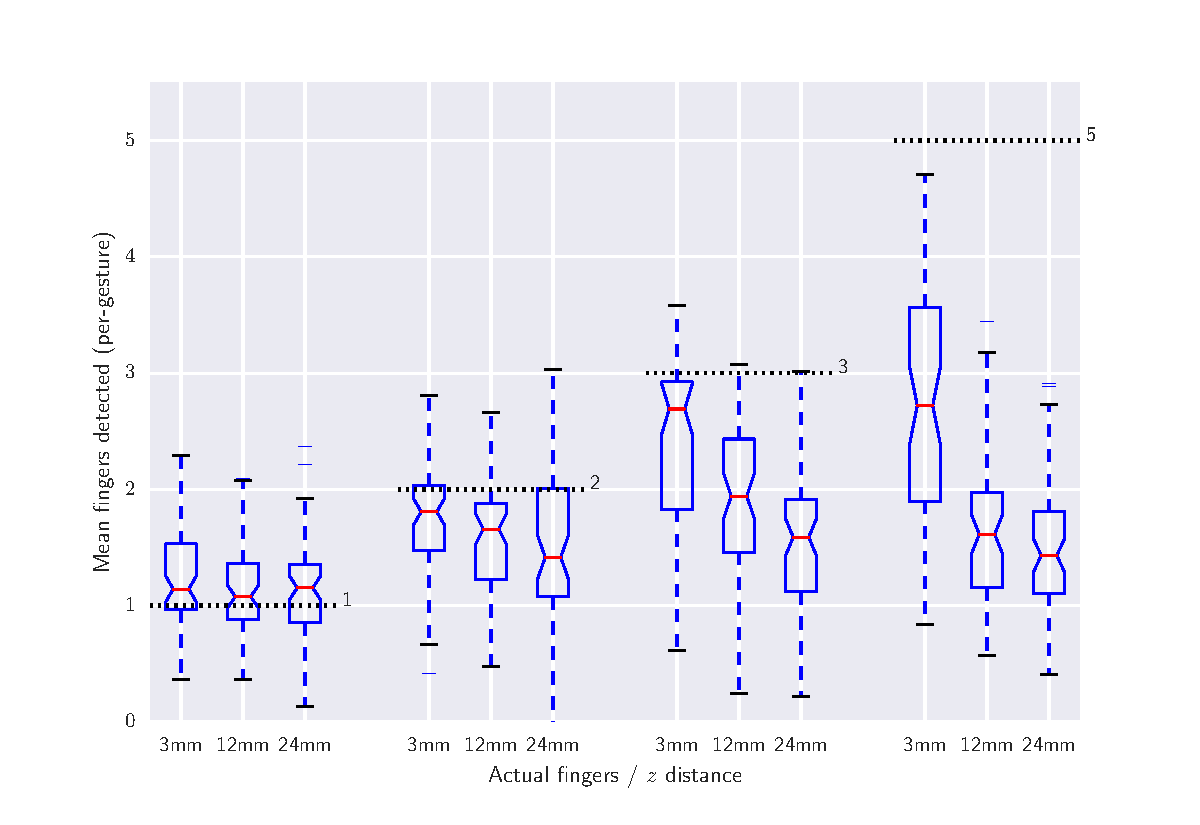
\includegraphics[width=1.0\linewidth]{images/boxplot_finger_distance.pdf}    

    \caption{Average number of fingers detected by the touch sensor at different heights above the surface, averaged over all gestures. Dashed lines indicate
    the true number of fingers present. The Box plots include bootstrapped uncertainty notches for the median. It is clear that the device is biased toward 
    undercounting fingers, particularly at higher $z$ distances.
    }

    % use the notation fig:name to cross reference a figure
    \label{fig:boxplot} 
\end{figure}


%==================================================================================================================================
\chapter{Conclusion}    
Summarise the whole project for a lazy reader who didn't read the rest (e.g. a prize-awarding committee).
\section{Guidance}
\begin{itemize}
    \item
        Summarise briefly and fairly.
    \item
        You should be addressing the general problem you introduced in the
        Introduction.        
    \item
        Include summary of concrete results (``the new compiler ran 2x
        faster'')
    \item
        Indicate what future work could be done, but remember: \textbf{you
        won't get credit for things you haven't done}.
\end{itemize}

%==================================================================================================================================
%
% 
%==================================================================================================================================
%  APPENDICES  

\begin{appendices}

\chapter{Appendices}

Typical inclusions in the appendices are:

\begin{itemize}
\item
  Copies of ethics approvals (required if obtained)
\item
  Copies of questionnaires etc. used to gather data from subjects.
\item
  Extensive tables or figures that are too bulky to fit in the main body of
  the report, particularly ones that are repetitive and summarised in the body.

\item Outline of the source code (e.g. directory structure), or other architecture documentation like class diagrams.

\item User manuals, and any guides to starting/running the software.

\end{itemize}

\textbf{Don't include your source code in the appendices}. It will be
submitted separately.

\end{appendices}

%==================================================================================================================================
%   BIBLIOGRAPHY   

% The bibliography style is abbrvnat
% The bibliography always appears last, after the appendices.

\bibliographystyle{abbrvnat}

\bibliography{l4proj}

\end{document}
